\documentclass{standalone}
%\documentclass[convert={outfile=\jobname.png}]{standalone}
\usepackage[utf8]{vietnam}
\usepackage{tikz}
\usetikzlibrary{calc,decorations.pathreplacing,angles,quotes}
\begin{document}
	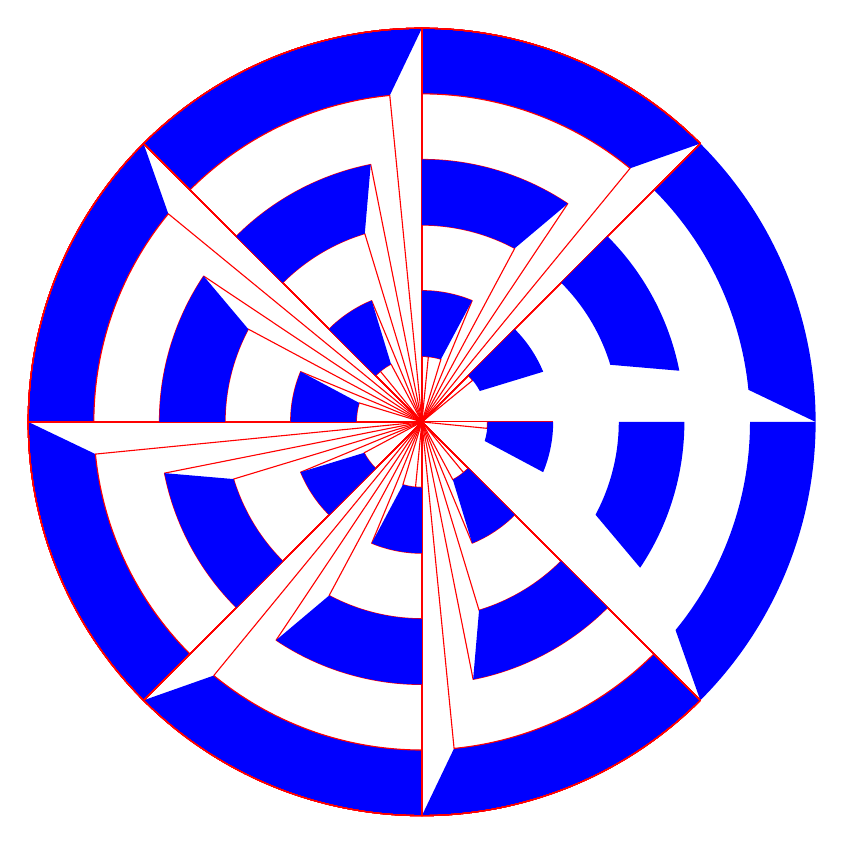
\begin{tikzpicture}[line join=round]
		\def\r{5}
		\def\n{6}
		\def\m{8}
		\colorlet{mau}{blue}
		\pgfmathsetmacro{\goc}{360/\m}
		\pgfmathsetmacro{\a}{\r/\n}
		\pgfmathsetmacro{\gochia}{\goc/\m}
		\coordinate (a) at (0:\r);
		\coordinate (b) at (\goc:\r);
		\pgfmathsetmacro{\bkm}{(\n-1)*\a}
		\foreach \i in {1,...,\m}{
			\pgfmathsetmacro{\gocm}{(\i -1)*\goc}
			\pgfmathsetmacro{\goch}{\i *\goc}
			\pgfmathsetmacro{\gochm}{\gocm+\gochia}
			\fill[color=mau] (\gocm:\r) arc (\gocm:\goch:\r) --(\goch:\bkm) arc (\goch:\gochm:\bkm)--cycle;
		}
		\foreach \i in {1,...,\m}{
			\foreach \j in {1,...,\n}{
				\pgfmathsetmacro{\Agm}{\i * \gochia}
				\pgfmathsetmacro{\Agh}{(\i +1)*\gochia}
				\pgfmathsetmacro{\rm}{(\n-\i) *\a}
				\pgfmathsetmacro{\rh}{(\n-\i-1)*\a}
				\pgfmathsetmacro{\quay}{\j *\goc}
				\draw[rotate=\quay,red] (0:0) --(\Agm:\rm) arc (\Agm :\goc:\rm);
				\draw[rotate=\quay,red] (0:0) -- (0:\r) arc (0:\goc:\r)--cycle;
			}
		}
		\pgfmathsetmacro{\tomau}{int((\n-2)/2)}
		\foreach \j in {1,...,\m}{
			\foreach \i in {1,...,\tomau}{
				\pgfmathsetmacro{\Agm}{(\j-1) * \goc+2*\i *\gochia}
				\pgfmathsetmacro{\Agh}{\j *\goc}
				\pgfmathsetmacro{\Aghm}{\Agm+\gochia}
				\pgfmathsetmacro{\rm}{(\n-2*\i) *\a}
				\pgfmathsetmacro{\rh}{(\n-2*\i-1)*\a}
				\fill[color=mau] (\Agm:\rm) arc (\Agm :\Agh:\rm) --(\Agh: \rh) arc(\Agh :\Aghm :\rh)--cycle;
			}
		}
	\end{tikzpicture}
\end{document}